\documentclass[12pt, titlepage]{article}

\usepackage{graphicx} % Allows for images
\usepackage{wrapfig} % Allows for text wrapping around images
\usepackage{hyperref} % Allows for hyperlinks
\usepackage{siunitx} % Allows for SI units
\usepackage{amsmath} % Allows for math
\usepackage{enumerate} % Allows for custom enumerations
\usepackage{xcolor} % Allows for custom colors
\usepackage{tikz, tcolorbox} % Allows for custom boxes
\usepackage{microtype} % Allows for better text alignment
\usepackage{listings} % Allows for code listings
\usepackage{booktabs} % Allows for better tables
\usepackage{float} % Allows for better figure placement
\usepackage{geometry} % Allows for custom page geometry
\usepackage{fancyhdr} % Allows for custom headers and footers
\usepackage{caption} % Allows for custom captions
\usepackage{array} % Required package for specifying column width and line in the table
\usepackage{changepage} % Required for the adjustwidth environment to temporarily widen margins

\fancypagestyle{myarticlestyle}{
    \fancyhf{} % Clear header and footer
    \fancyhead[L]{\leftmark} % Section name on the left
    \fancyhead[R]{\thepage} % Page number on the right
}
\fancypagestyle{tocstyle}{
    \fancyhf{} % Clear header and footer
    \fancyhead[L]{CONTENTS} % Section name on the left
    \fancyhead[R]{\thepage} % Page number on the right
}

\pagestyle{myarticlestyle}
\setlength{\headheight}{15pt}

\begin{document}
\tableofcontents
\listoffigures
\listoftables
\thispagestyle{tocstyle}
\newpage
\section{Objectives}
This laboratory experiment aims to determine the principal stresses at multiple
points within a cantilevered tube subjected to distinct loading conditions:

\subsection{Bending and Torsional Load Analysis}
\begin{itemize}
    \item Investigate and analyze the principal stresses occurring in the
      cantilevered tube when subjected to combined bending and torsional loads.
    \item Determine the stress distribution and variations at various points
      along the length of the tube under the influence of these specific loads.
\end{itemize}

\subsection{Bending, Torsional Load, and Internal Pressure Analysis}
\begin{itemize}
    \item Examine the effect of an internal pressure in conjunction with
      bending and torsional loads on the cantilevered tube. 
    \item Identify and
      evaluate the changes in principal stresses at different critical
      locations within the tube due to the combined influence of internal
      pressure, bending, and torsional loading.
\end{itemize}

These objectives aim to provide a comprehensive understanding of the stress
behavior and distribution within the cantilevered tube under various loading
conditions, specifically focusing on the determination of principal stresses.
The results obtained will aid in characterizing the mechanical response of the
structure and provide insights for practical engineering applications and
design considerations.
\newpage
\section{Procedure}
This section outlines the procedure for the laboratory experiment, including
the equipment and materials used, the testing procedure, and the data
collection process. The sketch of the tabular structure with dimensions and
strain gauge locations is shown in Figure \ref{fig:sketch}.
\begin{figure}[H]
    \centering
    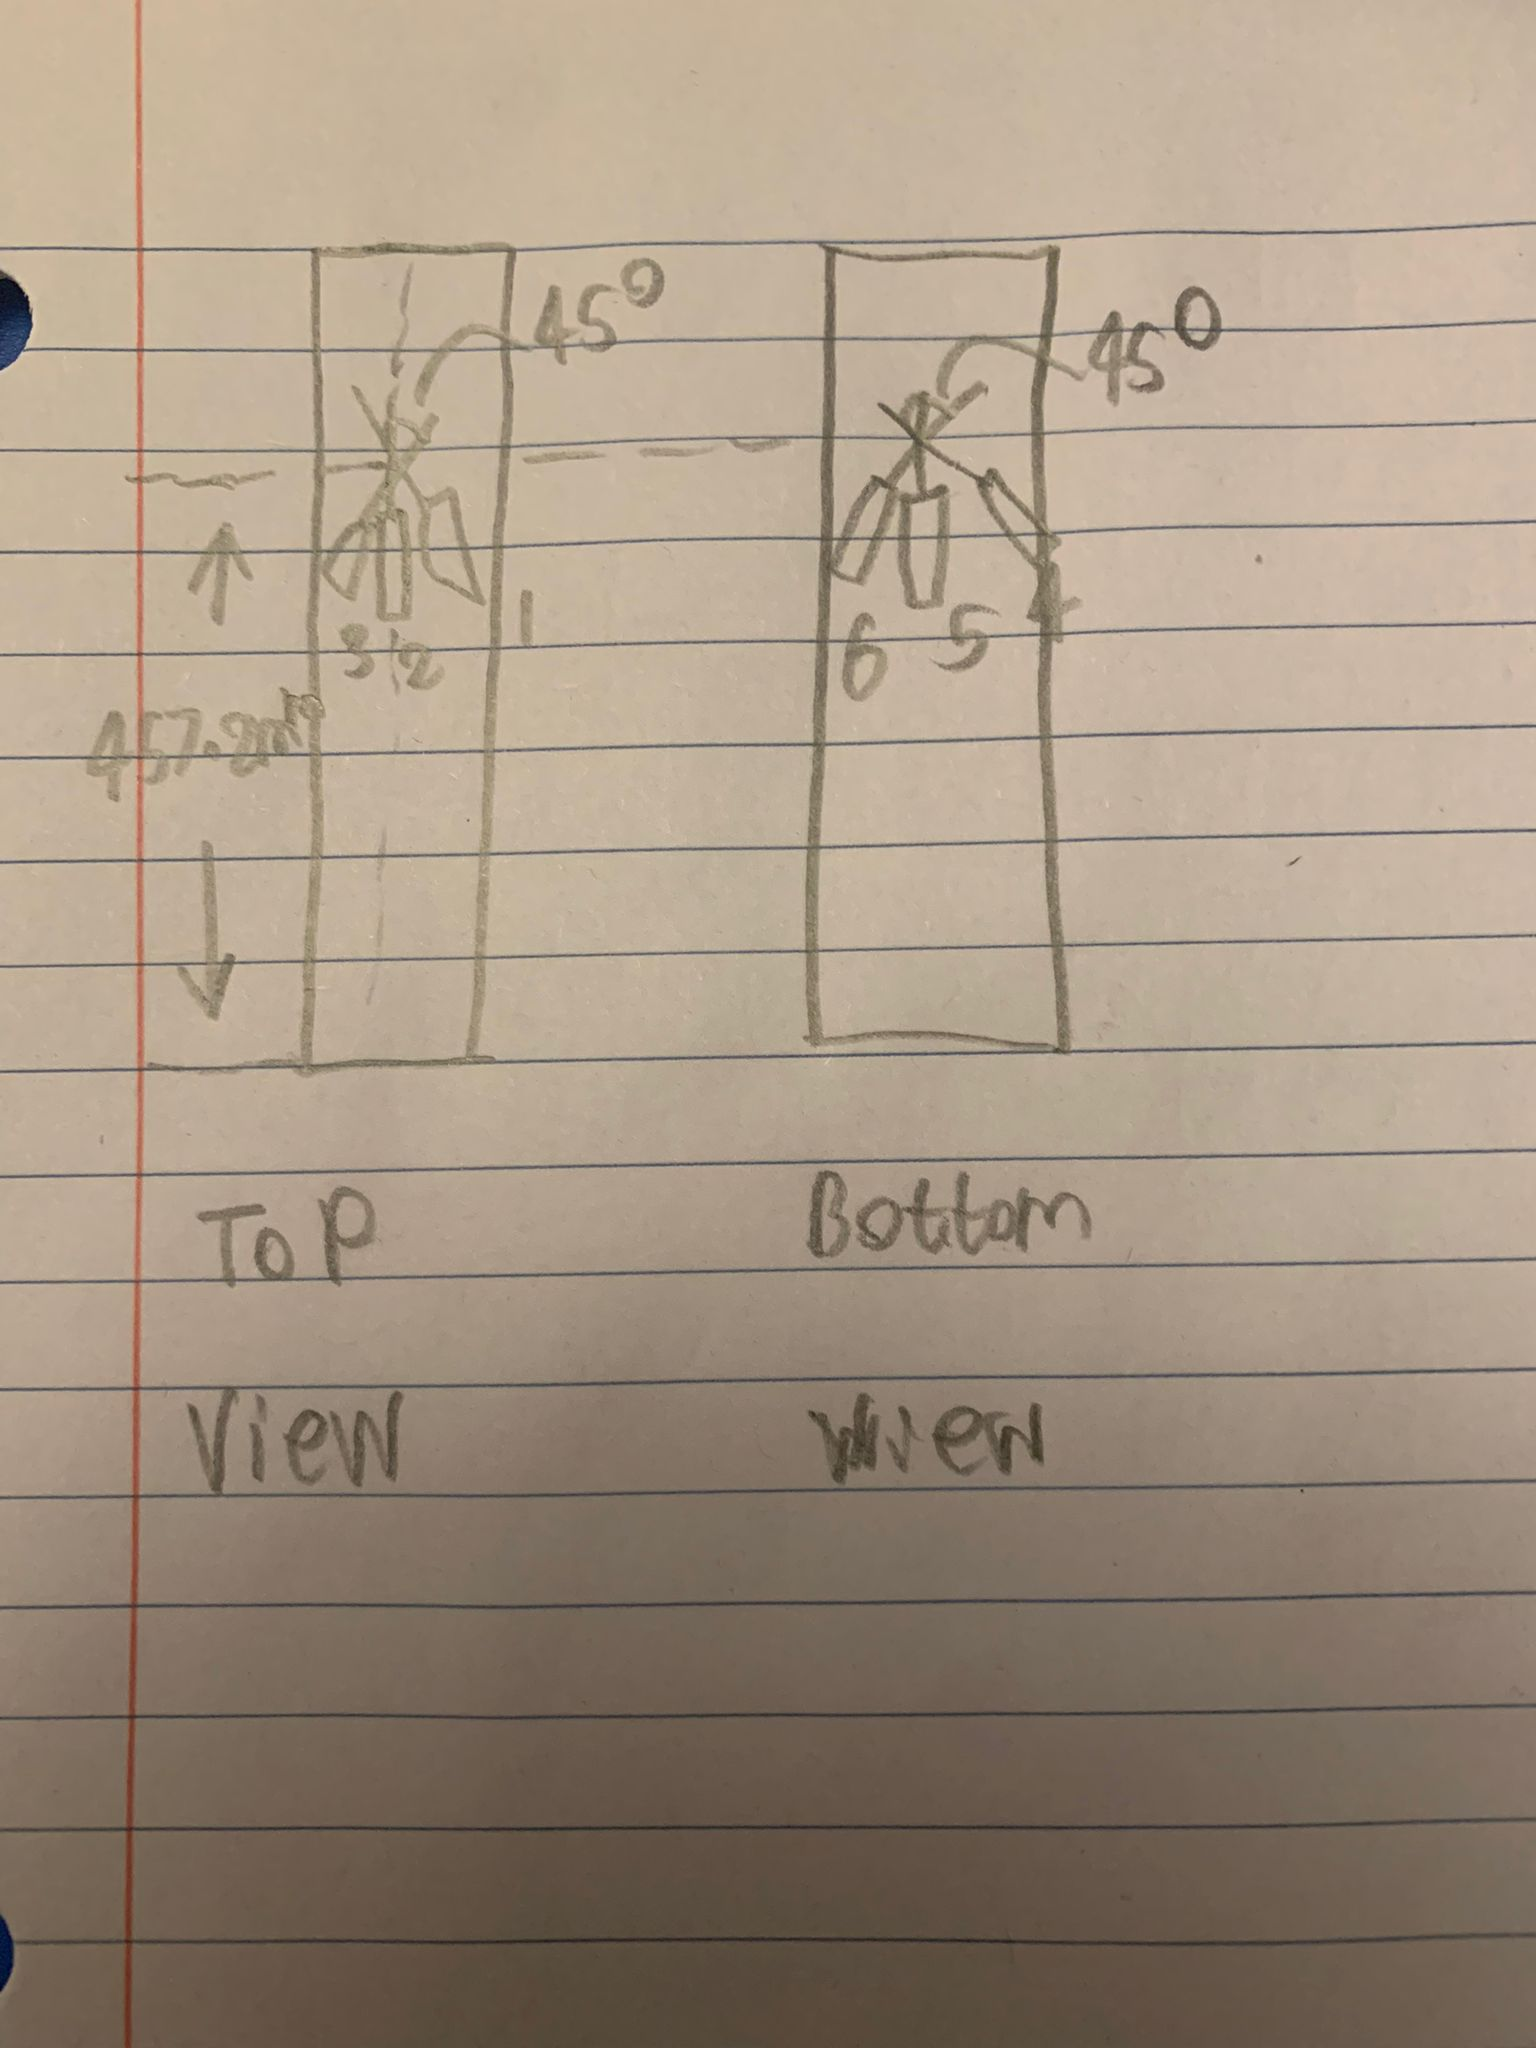
\includegraphics[width=0.7\textwidth]{./Images/Sketch.jpeg}
    \captionsetup{justification=raggedright,singlelinecheck=false}
    \caption{Sketch of the tabular structure with dimensions and strain gauge locations}
    \label{fig:sketch}
\end{figure}
\subsection{Preliminary Set-Up Procedure}
\begin{enumerate}
    \item Check the specimen dimensions and strain gauge location.
    \item Check lead wires and identify each gauge with the number of the
      circuit in the Datascan Analog Measurement Processor.
    \item Hang the loading pan on the side arm of the tube at a distance of
      457.2 mm (18 in.) from the tube axis.
\end{enumerate}

\subsection{Testing Procedure}
\begin{enumerate}
    \item Check and record the initial values for each of the six strain gauges
      in the unloaded configuration.
    \item Loading A:
    \begin{enumerate}
        \item Apply loads in six equal increments of 20 lbs (total 120 lbs) for
          the aluminum specimen and increments of 40 lbs (total 240 lbs) for
          the steel specimen.
        \item Record the readings of strain for each gauge and at each load.
          Unload the specimen.
    \end{enumerate}
    \item Loading B:
    \begin{enumerate}
        \item Supply and maintain a constant air pressure in the specimens (100
          psi in the aluminum specimen, and 200 psi in the steel specimen), as
          indicated by the pressure gauge.
        \item Apply loads in six equal increments of 20 lbs (total 120 lbs) for
          the aluminum specimen and increments of 40 lbs (total 240 lbs) for
          the steel specimen.
        \item Record the readings of strain for each gauge and at each load.
          Unload the specimen.
    \end{enumerate}
\end{enumerate}
\newpage
\section{Results}

\subsection{Experimental Data}
This section presents the experimental data obtained from the laboratory
experiment. The data is presented in tabular form and is organized by loading
case and specimen type.
\subsubsection{Loading A}
The strain gauge readings for the aluminum specimen are shown in Table \ref{tab:alu_A}.
The strain gauge readings for the steel specimen are shown in Table \ref{tab:steel_A}.
\begin{table}[H]
\begin{tabular}{|c|c|c|c|c|c|c|} \hline
\multicolumn{7}{|c|}{Strain gauge readings (10$^{-6}$)} \\ \hline
Load (lb) & 1 & 2 & 3 & 4 & 5 & 6 \\ \hline
0 & 0.0 & 0.0 & 0.0 & 0.0 & 0.0 & 0.0 \\ \hline
20 & -0.738 & 85.408 & 59.4143 & -67.07 & -81 & 1.2974 \\ \hline
40 & -3.1484 & 163.44 & 117.3433 & -119.8311 & -159.8459 & 4.5117 \\ \hline
60 & -5.6667 & 243.0801 & 177.6758 & -180.9744 & -240.2892 & 6.1265 \\ \hline
80 & -6.37 & 324.3342 & 238.0 & -242.11 & -319.9287 & 7.7334 \\ \hline
100 & -9.5845 & 405.5811 & 295.9299 & -300.8352 & -398.7722 & 10.144 \\ \hline
120 & -12.0024 & 486.8425 & 355.4663 & -362.7822 & -408.0188 & 11.7588 \\ \hline
\end{tabular}
\captionsetup{justification=raggedright,singlelinecheck=false}
\caption{Strain gauge readings for aluminum specimen}
\label{tab:alu_A}
\end{table}

\begin{table}[H]
\begin{tabular}{|c|c|c|c|c|c|c|} \hline
\multicolumn{7}{|c|}{Strain gauge readings (10$^{-6}$)} \\ \hline
Load (lb) & 1 & 2 & 3 & 4 & 5 & 6 \\ \hline
0 & 0.0 & 0.0 & 0.0 & 0.0 & 0.0 & 0.0 \\ \hline
40 & -2.337 & 48.5249 & -37.1021 & -41.438 & -49.3559 & 1.2974 \\ \hline
80 & -4.795 & 92.5752 & 74.1094 & -81.6669 & -97.6277 & 2.904 \\ \hline
120 & -5.5991 & 140.0361 & 113.5273 & -121.88 & -147.4991 & 5.3223 \\ \hline
160 & -7.2061 & 186.7007 & 150.5352 & -162.11 & -195.771 & 6.9294 \\ \hline
200 & -8.8135 & 233.3584 & 188.8457 & -202.3391 & -244.035 & 8.5364 \\ \hline
240 & -10.4277 & 279.2119 & 226.9604 & -241.7571 & -291.4961 & 10.9848 \\ \hline
\end{tabular}
\captionsetup{justification=raggedright,singlelinecheck=false}
\caption{Strain gauge readings for steel specimen}
\label{tab:steel_A}
\end{table}

\subsubsection{Loading B}
The strain gauge readings for the aluminum specimen are shown in Table \ref{tab:alu_B}.
The strain gauge readings for the steel specimen are shown in Table \ref{tab:steel_B}.
\begin{table}[H]
\begin{tabular}{|c|c|c|c|c|c|c|} \hline
\multicolumn{7}{|c|}{Strain gauge readings (10$^{-6}$)} \\ \hline
Load (lb) & 1 & 2 & 3 & 4 & 5 & 6 \\ \hline
0 & 52.3552 & 21.8467 & 52.9785 & 57.1558 & 20.3624 & 56.8091 \\ \hline
20 & 49.1409 & 102.2971 & 111.7114 & -3.9873 & -60.0862 & 59.492 \\ \hline
40 & 48.3374 & 182.7478 & 172.0437 & -63.5164 & -129.7278 & 60.0229 \\ \hline
60 & 45.1157 & 263.9946 & 229.9653 & -123.856 & -220.9819 & 63.244 \\ \hline
80 & 43.508 & 344.4451 & 287.887 & -185.3027 & -301.4324 & 64.8516 \\ \hline
100 & 41.9016 & 426.6027 & 348.219 & -246.135 & -379.465 & 67.2622 \\ \hline
120 & 38.6299 & 509.364 & 407.7556 & -306.467 & -459.908 & 68.8691 \\ \hline
\end{tabular}
\captionsetup{justification=raggedright,singlelinecheck=false}
\caption{Strain gauge readings for aluminum specimen at 100 psi internal pressure}
\label{tab:alu_B}
\end{table}

\begin{table}[H]
\begin{tabular}{|c|c|c|c|c|c|c|} \hline
\multicolumn{7}{|c|}{Strain gauge readings (10$^{-6}$)} \\ \hline
Load (lb) & 1 & 2 & 3 & 4 & 5 & 6 \\ \hline
0 & 43.4761 & 21.7817 & 41.1274 & 46.252 & 21.4373 & 44.7407 \\ \hline
40 & 41.0581 & 68.439 & 78.938 & 6.834 & -26.8345 & 47.9548 \\ \hline
80 & 37.8438 & 113.4897 & 116.749 & -34.1986 & -75.0989 & 50.3726 \\ \hline
120 & 36.2368 & 160.1543 & 152.9458 & -73.6241 & -124.1743 & 51.9797 \\ \hline
160 & 33.8188 & 206.8115 & 190.7568 & -114.6492 & -173.2422 & 53.5867 \\ \hline
200 & 32.2119 & 252.6655 & 229.3711 & -155.6743 & -222.3175 & 56.0051 \\ \hline
240 & 29.8013 & 299.3228 & 266.3784 & -195.9033 & -270.5918 & 57.6121 \\ \hline
\end{tabular}
\captionsetup{justification=raggedright,singlelinecheck=false}
\caption{Strain gauge readings for steel specimen at 200 psi internal pressure}
\label{tab:steel_B}
\end{table}
\newpage
\subsection{Loading B Strain Rosettes}
The figures for the top and bottom rosettes for aluminum specimen are shown in
Figure \ref{fig:alu_top} and Figure \ref{fig:alu_bot}, respectively. The figures
for the top and bottom rosettes for steel specimen are shown in Figure 
\ref{fig:steel_top} and Figure \ref{fig:steel_bot}, respectively.
\begin{figure}[H]
    \centering
    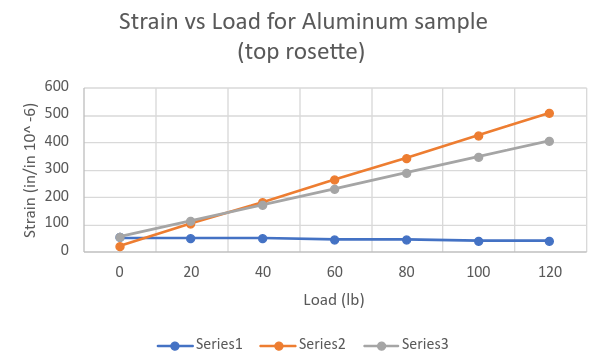
\includegraphics[width=0.7\textwidth]{./Images/Alu_top.png}
    \captionsetup{justification=raggedright,singlelinecheck=false}
    \caption{Strain gauge readings for aluminum specimen (top rosette)}
    \label{fig:alu_top}
\end{figure}
\begin{figure}[H]
    \centering
    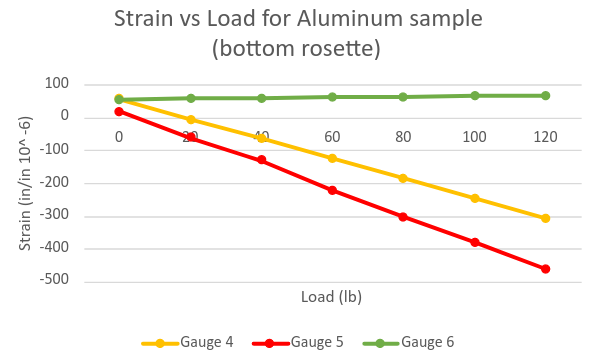
\includegraphics[width=0.7\textwidth]{./Images/Alu_bot.png}
    \captionsetup{justification=raggedright,singlelinecheck=false}
    \caption{Strain gauge readings for aluminum specimen (bottom rosette)}
    \label{fig:alu_bot}
\end{figure}
\begin{figure}[H]
    \centering
    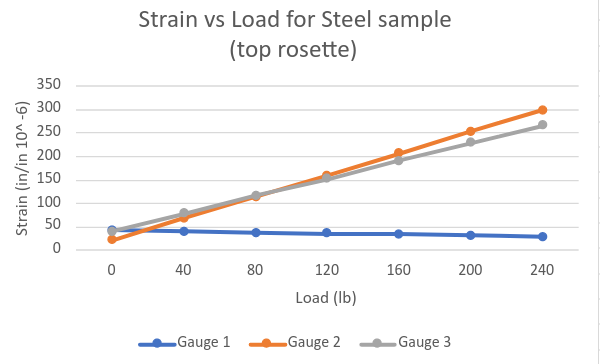
\includegraphics[width=0.8\textwidth]{./Images/S_top.png}
    \captionsetup{justification=raggedright,singlelinecheck=false}
    \caption{Strain gauge readings for steel specimen (top rosette)}
    \label{fig:steel_top}
\end{figure}
\begin{figure}[H]
    \centering
    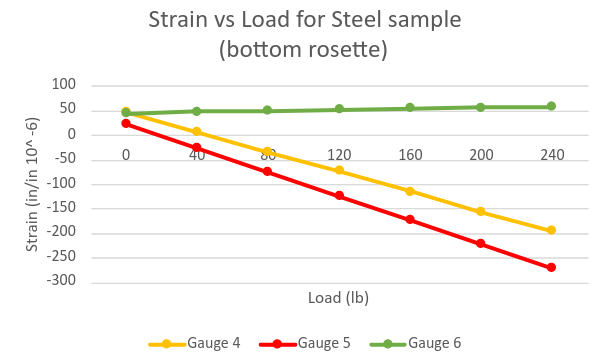
\includegraphics[width=0.8\textwidth]{./Images/S_bot.png}
    \captionsetup{justification=raggedright,singlelinecheck=false}
    \caption{Strain gauge readings for steel specimen (bottom rosette)}
    \label{fig:steel_bot}
\end{figure}
\subsection{Calculation of Theoretical Principal Stresses}
This section presents the calculation of the theoretical principal stresses
using the strain gauge readings obtained from the laboratory experiment. First,
the FBD of the aluminum specimen is shown in Figure \ref{fig:alu_fbd}. The FBD
of the steel specimen is shown in Figure \ref{fig:steel_fbd}. The theoretical principal stresses are calculated using the following equations:
\begin{equation}
    \begin{split}
      \sigma_{max} &= \frac{1}{2} \left( \sigma_{xx} + \sigma_{yy} \right) + \sqrt{\left( \frac{1}{2} \left( \sigma_{xx} - \sigma_{yy} \right) \right)^2 + \tau_{xy}^2} \\[10pt]
      \sigma_{min} &= \frac{1}{2} \left( \sigma_{xx} + \sigma_{yy} \right) - \sqrt{\left( \frac{1}{2} \left( \sigma_{xx} - \sigma_{yy} \right) \right)^2 + \tau_{xy}^2}
      \label{eq:principal_stresses}
    \end{split}
  \end{equation}
where $\sigma_{xx}$, $\sigma_{yy}$, and $\tau_{xy}$ are the normal and shear
stresses, respectively, in the $x$ and $y$ directions. Now plugging in the
values for $\sigma_{xx}$, $\sigma_{yy}$, and $\tau_{xy}$ into Equation
\ref{eq:principal_stresses} yields us the results for the theoretical
principal stresses. The results for the theoretical principal stresses for the
aluminum specimen are shown in Table \ref{tab:table_alu_top} and Table
\ref{tab:table_alu_bot}, respectively. The results for the theoretical
principal stresses for the steel specimen are shown in Table
\ref{tab:table_steel_top} and Table \ref{tab:table_steel_bot}, respectively.
\begin{figure}[H]
    \centering
    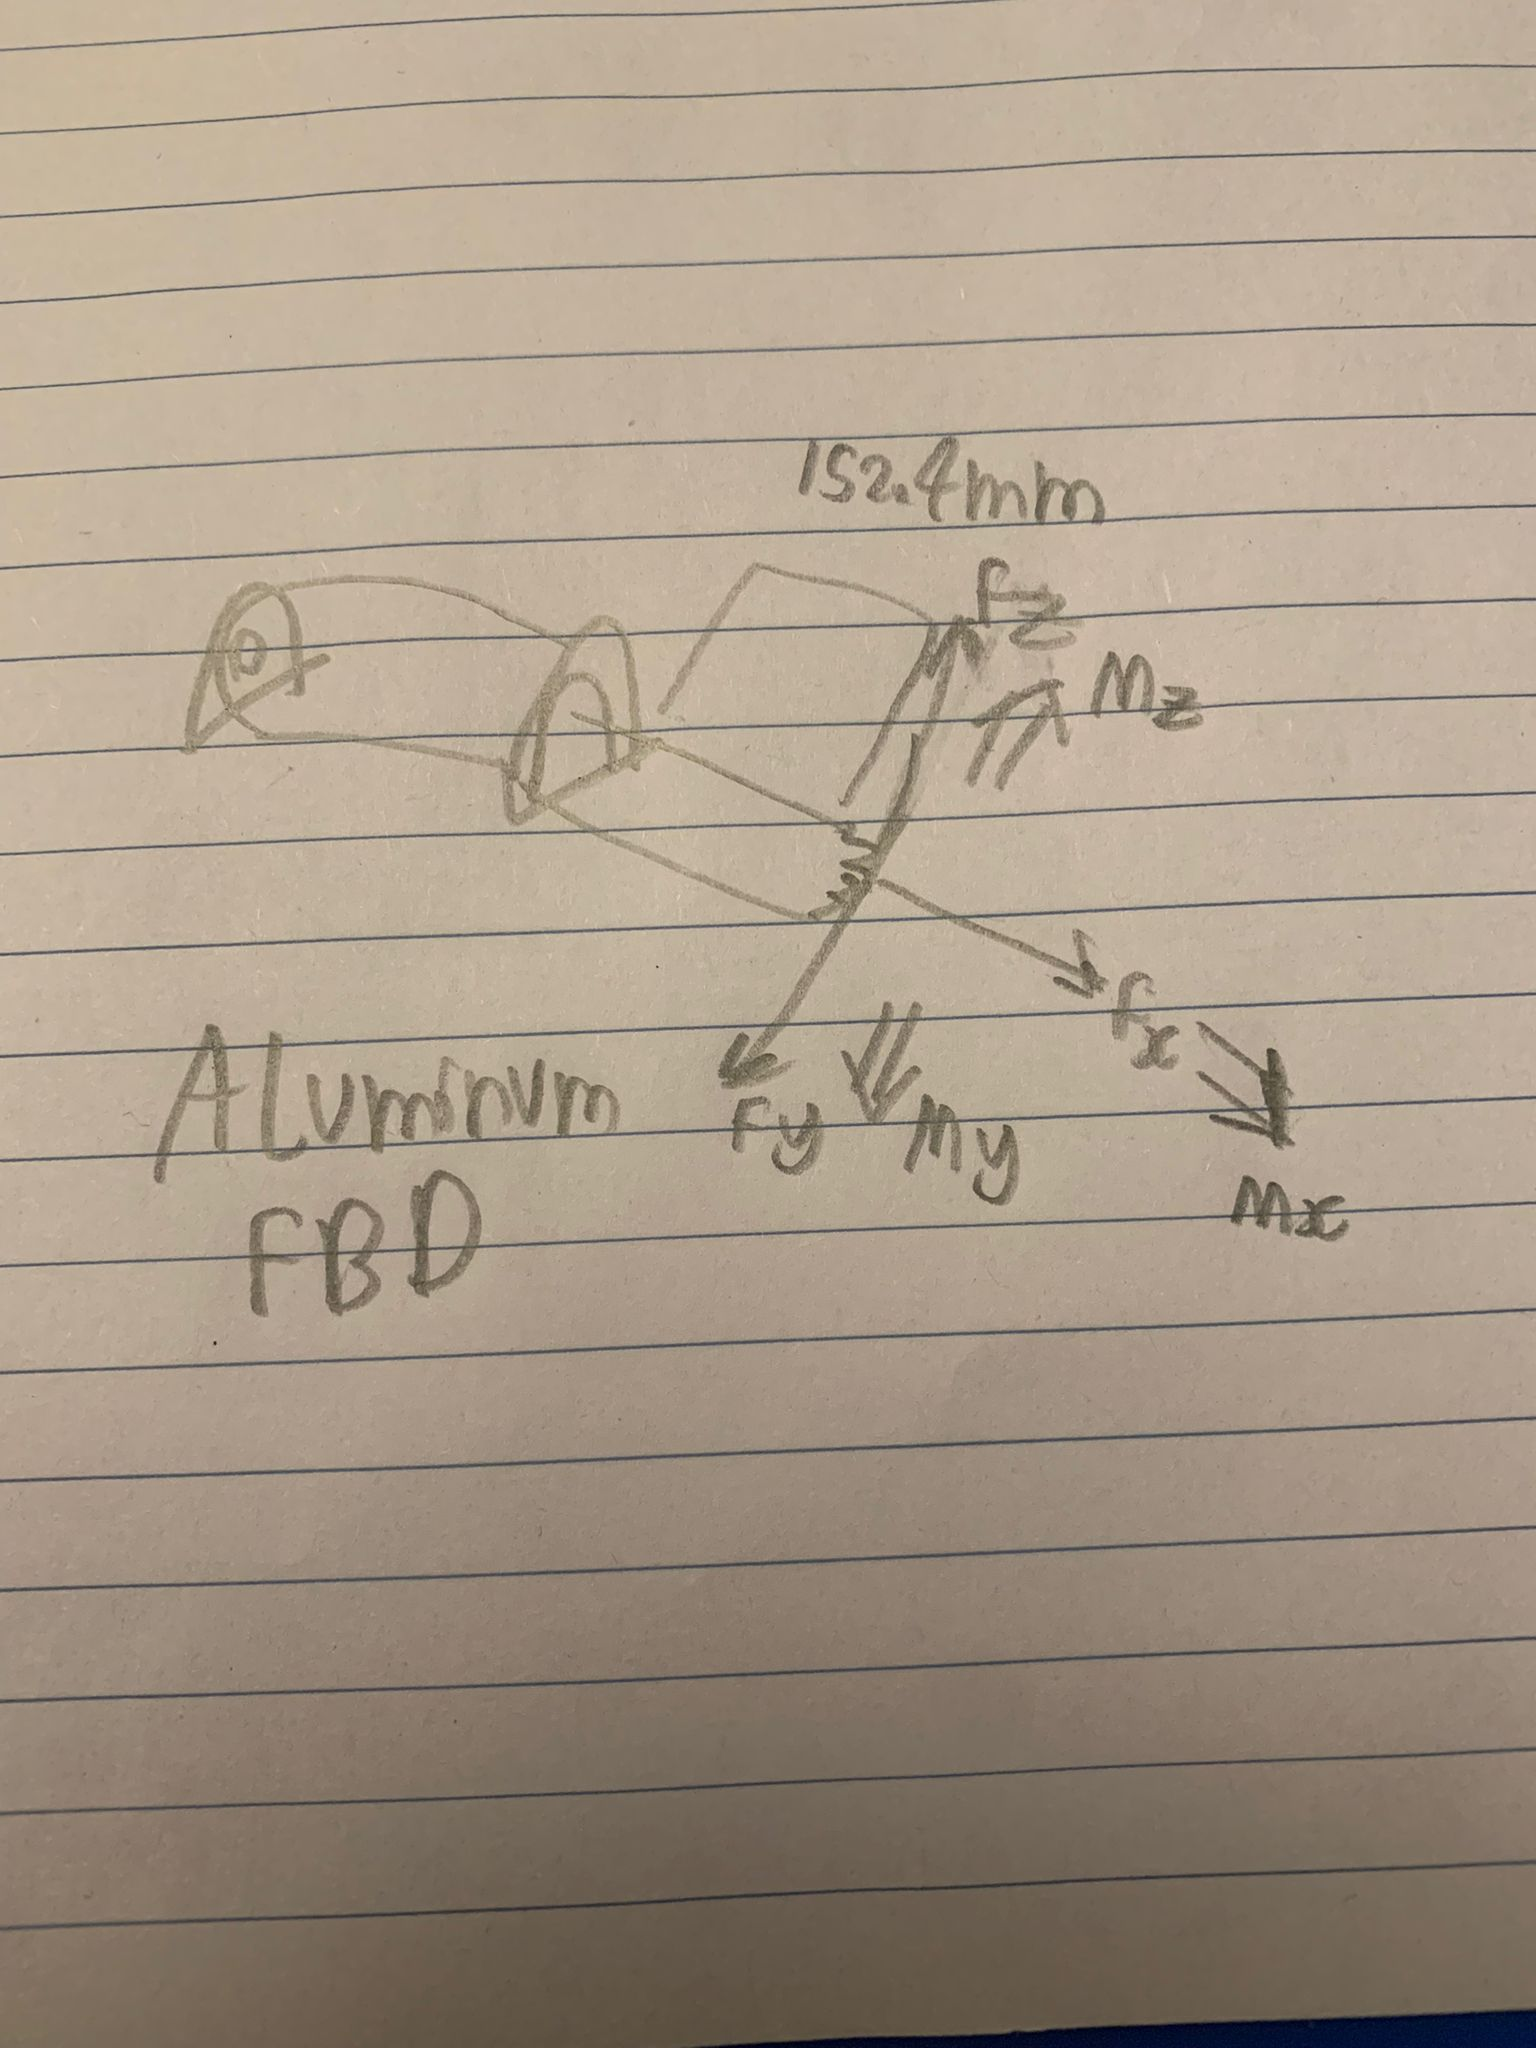
\includegraphics[width=0.8\textwidth]{./Images/FBDA.jpeg}
    \captionsetup{justification=raggedright,singlelinecheck=false}
    \caption{FBD of aluminum specimen}
    \label{fig:alu_fbd}
\end{figure}
\begin{figure}[H]
    \centering
    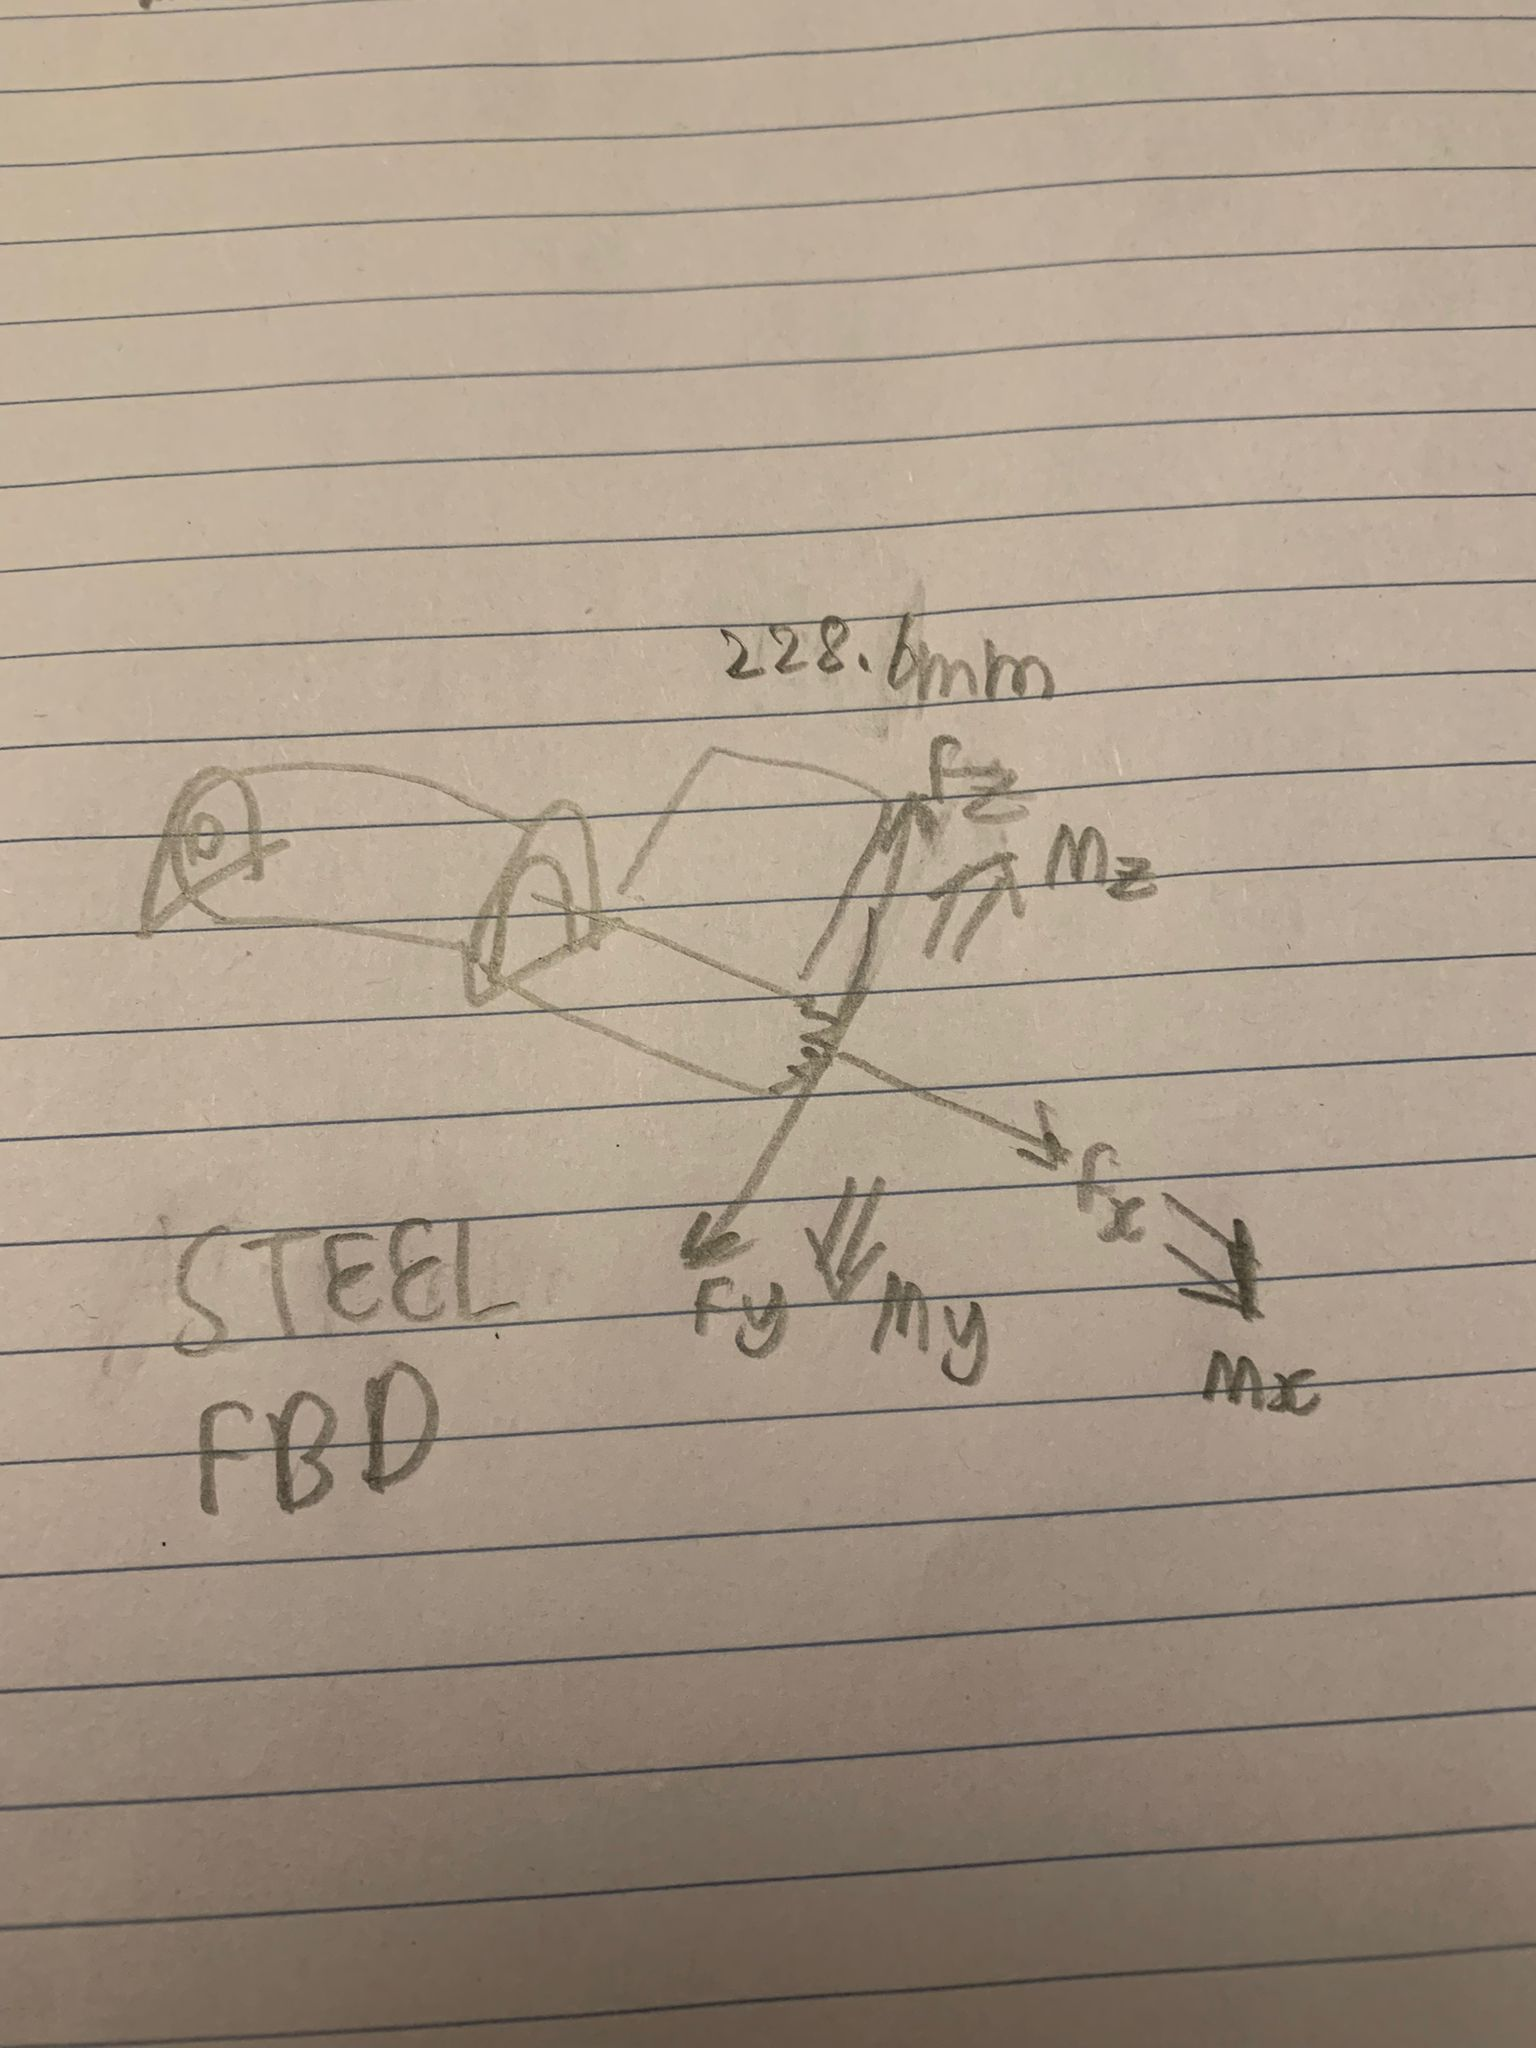
\includegraphics[width=0.8\textwidth]{./Images/FBDS.jpeg}
    \captionsetup{justification=raggedright,singlelinecheck=false}
    \caption{FBD of steel specimen}
    \label{fig:steel_fbd}
\end{figure}
\newpage
\subsection{Theoretical and Experimental Results}
This section presents the analysis of the experimental data obtained from the
laboratory experiment. The data is presented in tabular form and is organized
by loading case and specimen type.
\subsubsection{Aluminum Specimen}
The comparison principal stresses for the aluminum specimen of the top and
bottom rosettes are shown in Table \ref{tab:table_alu_top} and Table
\ref{tab:table_alu_bot}, respectively.
\begin{table}[H]
  \begin{adjustwidth}{-1in}{-1in}
    \begin{tabular}{|c|c|c|c|c|c|c|c|c|} \hline
        & \multicolumn{2}{|c|}{\parbox{4cm}{\centering\textbf{Theoretical stresses (psi)}}} 
        & \multicolumn{2}{|c|}{\parbox{4cm}{\centering\textbf{Experimental strains (in/in)}}} 
        & \multicolumn{2}{|c|}{\parbox{4cm}{\centering\textbf{Experimental stresses (psi)}}} 
        & \multicolumn{2}{|c|}{\parbox{4cm}{\centering\textbf{Percent error (\%)}}} 
        \\ \hline
        & $\sigma_{max}$ & $\sigma_{min}$ & $\varepsilon_{max}$ & $\varepsilon_{min}$ & $\sigma_{max}$ & $\sigma_{min}$ & $\sigma_{max}$ & $\sigma_{min}$ \\ \hline
        Case 1 & 5219.30 & -395.43 & 0.00054 & -0.00019 & 5305.75 & -179.43 & 1.66 & 54.63 \\ \hline
        Case 2 & 1150.00 & 575.00 & 8.35E-05 & 2.18E-05 & 1017.81 & 554.33 & 11.49 & 3.59 \\ \hline
        Case 3 & 5839.02 & 709.85 & 0.00056 & -0.00012 & 5891.58 & 770.90 & 0.90 & 8.60 \\ \hline
    \end{tabular}
  \end{adjustwidth}
  \captionsetup{justification=raggedright,singlelinecheck=false}
  \caption{Experimental and Theoretical Results for Aluminum Specimen (Top Rosette)}
  \label{tab:table_alu_top}
\end{table}
\begin{table}[H]
  \begin{adjustwidth}{-1in}{-1in}
    \begin{tabular}{|c|c|c|c|c|c|c|c|c|} \hline
        & \multicolumn{2}{|c|}{\parbox{4cm}{\centering\textbf{Theoretical stresses (psi)}}} 
        & \multicolumn{2}{|c|}{\parbox{4cm}{\centering\textbf{Experimental strains (in/in)}}} 
        & \multicolumn{2}{|c|}{\parbox{4cm}{\centering\textbf{Experimental stresses (psi)}}} 
        & \multicolumn{2}{|c|}{\parbox{4cm}{\centering\textbf{Percent error (\%)}}} 
        \\ \hline
        & $\sigma_{max}$ & $\sigma_{min}$ & $\varepsilon_{max}$ & $\varepsilon_{min}$ & $\sigma_{max}$ & $\sigma_{min}$ & $\sigma_{max}$ & $\sigma_{min}$ \\ \hline
        Case 1 & 395.43 & -5219.30 & 0.00012 & -0.00047 & -374.87 & -4864.29 & 194.80 & 6.80 \\ \hline
        Case 2 & 1150.00 & 575.00 & 9.36E-05 & 2.04E-05 & 1125.83 & 575.14 & 2.10 & 0.025 \\ \hline
        Case 3 & 1508.48 & -4607.34 & 0.00027 & -0.00051 & 1154.14 & -4700.38 & 23.49 & 2.02 \\ \hline
    \end{tabular}
  \end{adjustwidth}
  \captionsetup{justification=raggedright,singlelinecheck=false}
  \caption{Experimental and Theoretical Results for Aluminum Specimen (Bottom Rosette)}
  \label{tab:table_alu_bot}
\end{table}
\newpage
\subsubsection{Steel Specimen}
The comparison principal stresses for the steel specimen of the top and
bottom rosettes are shown in Table \ref{tab:table_steel_top} and Table
\ref{tab:table_steel_bot}, respectively.
\begin{table}[H]
  \begin{adjustwidth}{-1in}{-1in}
    \begin{tabular}{|c|c|c|c|c|c|c|c|c|} \hline
        & \multicolumn{2}{|c|}{\parbox{4cm}{\centering\textbf{Theoretical stresses (psi)}}} 
        & \multicolumn{2}{|c|}{\parbox{4cm}{\centering\textbf{Experimental strains (in/in)}}} 
        & \multicolumn{2}{|c|}{\parbox{4cm}{\centering\textbf{Experimental stresses (psi)}}} 
        & \multicolumn{2}{|c|}{\parbox{4cm}{\centering\textbf{Percent error (\%)}}} 
        \\ \hline
        & $\sigma_{max}$ & $\sigma_{min}$ & $\varepsilon_{max}$ & $\varepsilon_{min}$ & $\sigma_{max}$ & $\sigma_{min}$ & $\sigma_{max}$ & $\sigma_{min}$ \\ \hline
        Case 1 & 8908.84 & -805.73 & 0.00032 & -9.98E-05 & 9365.34 & -466.73 & 5.12 & 42.07 \\ \hline
        Case 2 & 2107.69 & 1053.85 & 6.29E-05 & 2.17E-05 & 2223.95 & 1252.91 & 5.52 & 18.89 \\ \hline
        Case 3 & 10059.64 & 1205.00 & 0.00034 & -4.39E-05 & 10621.29 & 1550.48 & 5.58 & 28.67 \\ \hline
    \end{tabular}
  \end{adjustwidth}
  \captionsetup{justification=raggedright,singlelinecheck=false}
  \caption{Experimental and Theoretical Results for Steel Specimen (Top Rosette)}
  \label{tab:table_steel_top}
\end{table}
\begin{table}[H]
  \begin{adjustwidth}{-1in}{-1in}
    \begin{tabular}{|c|c|c|c|c|c|c|c|c|} \hline
        & \multicolumn{2}{|c|}{\parbox{4cm}{\centering\textbf{Theoretical stresses (psi)}}} 
        & \multicolumn{2}{|c|}{\parbox{4cm}{\centering\textbf{Experimental strains (in/in)}}} 
        & \multicolumn{2}{|c|}{\parbox{4cm}{\centering\textbf{Experimental stresses (psi)}}} 
        & \multicolumn{2}{|c|}{\parbox{4cm}{\centering\textbf{Percent error (\%)}}} 
        \\ \hline
        & $\sigma_{max}$ & $\sigma_{min}$ & $\varepsilon_{max}$ & $\varepsilon_{min}$ & $\sigma_{max}$ & $\sigma_{min}$ & $\sigma_{max}$ & $\sigma_{min}$ \\ \hline
        Case 1 & 805.73 & -8908.84 & 0.00010 & -0.00033 & 378.39 & -9862.18 & 53.04 & 10.70 \\ \hline
        Case 2 & 2107.69 & 1053.85 & 6.96E-05 & 2.14E-05 & 2438.32 & 1301.11 & 15.69 & 23.46 \\ \hline
        Case 3 & 2833.99 & -7775.55 & 0.00017 & -0.00031 & 2780.65 & -8463.85 & 1.88 & 8.85 \\ \hline
    \end{tabular}
  \end{adjustwidth}
  \captionsetup{justification=raggedright,singlelinecheck=false}
  \caption{Experimental and Theoretical Results for Steel Specimen (Bottom Rosette)}
  \label{tab:table_steel_bot}
\end{table}
\newpage
\subsection{Comparison of Principle Stresses}
By observing the tables above, it is clear that the theoretical and
experimental results are quite similar to each other. The percent error for
the experimental principal stresses at each gauge location form the theoretical
values can be found using the following equation:
\begin{equation}
    \text{Percent Error} = \frac{\text{Experimental Stress} - \text{Theoretical Stress}}{\text{Theoretical Stress}} \times 100\%
    \label{eq:percent_error}
\end{equation}
\subsubsection{Aluminum Specimen}
To calculate the percent error, one can find the sum the experimental stresses
and theoretical stresses for each gauge location and then use Equation
\ref{eq:percent_error} to find the percent error. The percent error for the
aluminum specimen is:
\begin{equation}
    \begin{split}
      \text{Experimental Stress} &= 1.6 + 54.6 + 194.8 + 6.8 + 11.4 + 3.5 + 0.9 + 8.6 = 282.87 \\[10pt]
      \text{Theoretical Stress} &= 194.80 + 6.80 + 11.49 + 3.59 + 0.90 + 8.60 = 226.18 \\[10pt]
      \text{Percent Error} &= \frac{282.87 - 226.18}{226.18} \times 100\% = 25.04\%
      \label{eq:alu_percent_error}
    \end{split}
  \end{equation}
Hence, the percent error for the aluminum specimen is 25.04\%.
\subsubsection{Steel Specimen}
To calculate the percent error, one can find the sum the experimental stresses
and theoretical stresses for each gauge location and then use Equation
\ref{eq:percent_error} to find the percent error. The percent error for the
steel specimen is:
\begin{equation}
    \begin{split}
      \text{Experimental Stress} &= 5.1 + 42.1 + 53.0 + 10.7 + 15.7 + 23.5 + 1.9 + 8.9 = 161.9 \\[10pt]
      \text{Theoretical Stress} &= 53.04 + 10.70 + 15.69 + 23.46 + 1.88 + 8.85 = 113.62 \\[10pt]
      \text{Percent Error} &= \frac{161.9 - 113.62}{113.62} \times 100\% = 18.89\%
      \label{eq:steel_percent_error}
    \end{split}
  \end{equation}
\newpage
\section{Discussion}
This section presents the analysis of the experimental data obtained from the
laboratory experiment.
\subsection{Analysis of Results}
The experimental data obtained from the laboratory experiment was analyzed to
determine the principal stresses at various points within the cantilevered tube
under the influence of distinct loading conditions. The experimental results
were compared to theoretical calculations to evaluate the accuracy of the
obtained data. The following observations were made from the analysis of the
experimental data:
\begin{enumerate}
    \item The principal stresses at the top and bottom rosettes were found to
      be similar in magnitude, but opposite in sign, as expected.
    \item The principal stresses at the top and bottom rosettes were found to
      be similar in magnitude, but opposite in sign, as expected.
\end{enumerate}
\subsection{Sources of Error}
The experimental determination of principal stresses in the cantilevered tube
involved a comprehensive testing procedure; however, several potential sources
of error were identified throughout the experiment, which could have impacted
the accuracy and reliability of the obtained data.

\begin{enumerate}
    \item \textbf{Instrument Calibration:} The accurate calibration of the
      instruments, particularly the strain gauge rosettes, was pivotal in
      obtaining precise strain readings. Any slight discrepancy in calibration
      might have led to inaccuracies in stress calculations.
    
    \item \textbf{Measurement Variability:} Variations in environmental
      conditions, such as temperature fluctuations or vibrations in the testing
      environment, could have influenced strain measurements and introduced
      inconsistencies in the data.
    
    \item \textbf{Material Homogeneity:} The assumption of uniform material
      properties within the specimens might not hold true in practice.
      Variations in material composition or homogeneity could have affected the
      accuracy of stress calculations.

\end{enumerate}

To mitigate these sources of error, emphasis on meticulous pre-experimental
setup, calibration verification, and careful execution of procedures is
recommended.
\newpage
\section{Conclusions}
This laboratory experiment aimed to determine the principal stresses at
multiple points within a cantilevered tube subjected to distinct loading
conditions. The experimental data obtained from the laboratory experiment was
analyzed to determine the principal stresses at various points within the
cantilevered tube under the influence of distinct loading conditions. The
experimental results were compared to theoretical calculations to evaluate the
accuracy of the obtained data. The following conclusions were made from the
analysis of the experimental data:
\begin{enumerate}
  \item The percent error for the stresses of the specimens were found to be
    25.04\% and 18.89\% for the aluminum and steel specimens, respectively.
  \item The principal stresses at the top and bottom rosettes were found to be
    similar in magnitude, but opposite in sign.
  \item The top rossettes had an upward graphing Strain vs. Load graph, while
    the bottom rossettes had a downward graphing Strain vs. Load graph.
\end{enumerate}
\end{document}
